% This file was converted to LaTeX by Writer2LaTeX ver. 1.4
% see http://writer2latex.sourceforge.net for more info
\documentclass[11pt]{article}
\usepackage[utf8]{inputenc}
\usepackage[T1]{fontenc}
\usepackage[french]{babel}
\usepackage{amsmath}
\usepackage{amssymb,amsfonts,textcomp}
\usepackage{array}
\usepackage{supertabular}
\usepackage{hhline}
\usepackage{hyperref}
\hypersetup{colorlinks=true, linkcolor=blue, citecolor=blue, filecolor=blue, urlcolor=blue}
\usepackage{graphicx}
% footnotes configuration
\makeatletter
\renewcommand\thefootnote{\arabic{footnote}}
\renewcommand\@makefnmark{\mbox{\textstyleFootnoteanchor{\@thefnmark}}}
\makeatother
\newcommand\textsubscript[1]{\ensuremath{{}_{\text{#1}}}}
% Text styles
\newcommand\textstyleFootnoteanchor[1]{\textsuperscript{#1}}
\makeatletter
\newcommand\arraybslash{\let\\\@arraycr}
\makeatother
\raggedbottom
% Paragraph styles
\renewcommand\familydefault{\rmdefault}
\newenvironment{styleStandard}{\renewcommand\baselinestretch{1.0}\setlength\leftskip{0cm}\setlength\rightskip{0cm plus 1fil}\setlength\parindent{0cm}\setlength\parfillskip{0pt plus 1fil}\setlength\parskip{0in plus 1pt}\writerlistparindent\writerlistleftskip\leavevmode\normalfont\normalsize\writerlistlabel\ignorespaces}{\unskip\vspace{0.111in plus 0.0111in}\par}
\newenvironment{styleListParagraph}{\renewcommand\baselinestretch{1.0}\setlength\leftskip{0.5in}\setlength\rightskip{0in plus 1fil}\setlength\parindent{0in}\setlength\parfillskip{0pt plus 1fil}\setlength\parskip{0in plus 1pt}\writerlistparindent\writerlistleftskip\leavevmode\normalfont\normalsize\writerlistlabel\ignorespaces}{\unskip\vspace{0.111in plus 0.0111in}\par}
\newenvironment{stylecaption}{\renewcommand\baselinestretch{1.0}\setlength\leftskip{0cm}\setlength\rightskip{0cm plus 1fil}\setlength\parindent{0cm}\setlength\parfillskip{0pt plus 1fil}\setlength\parskip{0in plus 1pt}\writerlistparindent\writerlistleftskip\leavevmode\normalfont\normalsize\fontsize{9pt}{10.8pt}\selectfont\itshape\writerlistlabel\ignorespaces}{\unskip\vspace{0.139in plus 0.0139in}\par}
% List styles
\newcommand\writerlistleftskip{}
\newcommand\writerlistparindent{}
\newcommand\writerlistlabel{}
\newcommand\writerlistremovelabel{\aftergroup\let\aftergroup\writerlistparindent\aftergroup\relax\aftergroup\let\aftergroup\writerlistlabel\aftergroup\relax}
\newcounter{listWWNumxxleveli}
\newcounter{listWWNumxxlevelii}[listWWNumxxleveli]
\newcounter{listWWNumxxleveliii}[listWWNumxxlevelii]
\newcounter{listWWNumxxleveliv}[listWWNumxxleveliii]
\renewcommand\thelistWWNumxxleveli{\arabic{listWWNumxxleveli}}
\renewcommand\thelistWWNumxxlevelii{\arabic{listWWNumxxleveli}.\arabic{listWWNumxxlevelii}}
\renewcommand\thelistWWNumxxleveliii{\arabic{listWWNumxxleveli}.\arabic{listWWNumxxlevelii}.\arabic{listWWNumxxleveliii}}
\renewcommand\thelistWWNumxxleveliv{\arabic{listWWNumxxleveli}.\arabic{listWWNumxxlevelii}.\arabic{listWWNumxxleveliii}.\arabic{listWWNumxxleveliv}}
\newcommand\labellistWWNumxxleveli{\thelistWWNumxxleveli.}
\newcommand\labellistWWNumxxlevelii{\thelistWWNumxxlevelii.}
\newcommand\labellistWWNumxxleveliii{\thelistWWNumxxleveliii.}
\newcommand\labellistWWNumxxleveliv{\thelistWWNumxxleveliv.}
\newenvironment{listWWNumxxleveli}{\def\writerlistleftskip{\setlength\leftskip{0.25in}}\def\writerlistparindent{}\def\writerlistlabel{}\def\item{\def\writerlistparindent{\setlength\parindent{-0.25in}}\def\writerlistlabel{\stepcounter{listWWNumxxleveli}\makebox[0cm][l]{\labellistWWNumxxleveli}\hspace{0.0cm}\writerlistremovelabel}}}{}
\newenvironment{listWWNumxxlevelii}{\def\writerlistleftskip{\setlength\leftskip{0.55in}}\def\writerlistparindent{}\def\writerlistlabel{}\def\item{\def\writerlistparindent{\setlength\parindent{-0.3in}}\def\writerlistlabel{\stepcounter{listWWNumxxlevelii}\makebox[0cm][l]{\labellistWWNumxxlevelii}\hspace{-0.635cm}\writerlistremovelabel}}}{}
\newenvironment{listWWNumxxleveliii}{\def\writerlistleftskip{\setlength\leftskip{0.85in}}\def\writerlistparindent{}\def\writerlistlabel{}\def\item{\def\writerlistparindent{\setlength\parindent{-0.35in}}\def\writerlistlabel{\stepcounter{listWWNumxxleveliii}\makebox[0cm][l]{\labellistWWNumxxleveliii}\hspace{-1.27cm}\writerlistremovelabel}}}{}
\newenvironment{listWWNumxxleveliv}{\def\writerlistleftskip{\setlength\leftskip{1.2in}}\def\writerlistparindent{}\def\writerlistlabel{}\def\item{\def\writerlistparindent{\setlength\parindent{-0.45in}}\def\writerlistlabel{\stepcounter{listWWNumxxleveliv}\makebox[0cm][l]{\labellistWWNumxxleveliv}\hspace{-1.9050001cm}\writerlistremovelabel}}}{}
\newcounter{listWWNumvileveli}
\newcounter{listWWNumvilevelii}[listWWNumvileveli]
\newcounter{listWWNumvileveliii}[listWWNumvilevelii]
\newcounter{listWWNumvileveliv}[listWWNumvileveliii]
\renewcommand\thelistWWNumvileveli{\arabic{listWWNumvileveli}}
\renewcommand\thelistWWNumvilevelii{\alph{listWWNumvilevelii}}
\renewcommand\thelistWWNumvileveliii{\roman{listWWNumvileveliii}}
\renewcommand\thelistWWNumvileveliv{\arabic{listWWNumvileveliv}}
\newcommand\labellistWWNumvileveli{(\thelistWWNumvileveli)}
\newcommand\labellistWWNumvilevelii{\thelistWWNumvilevelii.}
\newcommand\labellistWWNumvileveliii{\thelistWWNumvileveliii.}
\newcommand\labellistWWNumvileveliv{\thelistWWNumvileveliv.}
\newenvironment{listWWNumvileveli}{\def\writerlistleftskip{\setlength\leftskip{0.5in}}\def\writerlistparindent{}\def\writerlistlabel{}\def\item{\def\writerlistparindent{\setlength\parindent{-0.25in}}\def\writerlistlabel{\stepcounter{listWWNumvileveli}\makebox[0cm][l]{\labellistWWNumvileveli}\hspace{-0.635cm}\writerlistremovelabel}}}{}
\newenvironment{listWWNumvilevelii}{\def\writerlistleftskip{\setlength\leftskip{1in}}\def\writerlistparindent{}\def\writerlistlabel{}\def\item{\def\writerlistparindent{\setlength\parindent{-0.25in}}\def\writerlistlabel{\stepcounter{listWWNumvilevelii}\makebox[0cm][l]{\labellistWWNumvilevelii}\hspace{-1.905cm}\writerlistremovelabel}}}{}
\newenvironment{listWWNumvileveliii}{\def\writerlistleftskip{\setlength\leftskip{1.5in}}\def\writerlistparindent{}\def\writerlistlabel{}\def\item{\def\writerlistparindent{\setlength\parindent{-0.1252in}}\def\writerlistlabel{\stepcounter{listWWNumvileveliii}\makebox[0cm][r]{\labellistWWNumvileveliii}\hspace{-3.4919918cm}\writerlistremovelabel}}}{}
\newenvironment{listWWNumvileveliv}{\def\writerlistleftskip{\setlength\leftskip{2in}}\def\writerlistparindent{}\def\writerlistlabel{}\def\item{\def\writerlistparindent{\setlength\parindent{-0.25in}}\def\writerlistlabel{\stepcounter{listWWNumvileveliv}\makebox[0cm][l]{\labellistWWNumvileveliv}\hspace{-4.4449997cm}\writerlistremovelabel}}}{}
\setlength\tabcolsep{1mm}
\renewcommand\arraystretch{1.3}
\newcounter{Table}
\renewcommand\theTable{\arabic{Table}}
\newcommand\normalsubformula[1]{\text{\mathversion{normal}$#1$}}
\title{}
\author{}
\date{2020-04-08}
\begin{document}
\clearpage\setcounter{page}{1}\begin{styleStandard}
\textbf{Comparing ERPs between native speakers and second language learners: Dealing with individual variability}
\end{styleStandard}

\begin{styleStandard}
\textbf{Maud Pélissier, University of Agder}
\end{styleStandard}

\begin{styleStandard}
\textbf{Abstract }
\end{styleStandard}

\begin{styleStandard}
Event-related potentials (ERPs) are of great interest in second language acquisition research, as they allow us to examine online language processing and to compare the mechanisms that are engaged to process a first and second language. A long history of research into native language processing has taught us to expect a biphasic pattern in response to syntactic violations, reflecting mechanisms involved first in the automatic and implicit detection of the incongruity and then in the reanalysis and repair of the ungrammatical sentence. However, recent studies show that there is a large degree of individual variability even among native speakers: Instead of this biphasic pattern, most people exhibit one or the other of the two components. This raises an interesting question for second-language research: How do we compare learners and native speakers if there is no unique native-speaker model to compare learners to? In this chapter, I explore two measures that have been put forward to characterise individual variability among native speakers and language learners, the Response Magnitude Index and the Response Dominance Index (Tanner et al. 2014), and I show an example of their application to a study comparing native-speaker and non-native-speaker processing of morphosyntactic violations using auditory stimuli instead of visual stimuli.
\end{styleStandard}

\begin{styleStandard}
\textbf{Keywords}: ERPs; individual differences; second language learners; RMI; RDI
\end{styleStandard}


\setcounter{listWWNumxxleveli}{0}
\begin{listWWNumxxleveli}
\item 
\begin{styleListParagraph}
\textbf{Introduction}
\end{styleListParagraph}
\end{listWWNumxxleveli}
\begin{styleStandard}
A large part of research in second language acquisition (SLA) is devoted to comparing learners’ performance to native speakers’ performance, including measures of online and offline production and perception of a variety of more or less complex language structures, in order to see how learners may differ at various levels of proficiency. One of the fundamental questions in SLA research is whether learners can and do process their second language (L2) like native speakers (i.e., by engaging the same cognitive and cerebral mechanisms). The development of affordable imagery techniques like electroencephalography (EEG), which records the electric activity of the brain at the surface of the scalp, has given researchers a window into language processing in real time, as opposed to the more indirect measures provided by behavioural experiments. There is an abundant literature on whether L2 learners can eventually recruit the same cognitive mechanisms – as reflected by different event-related potential (ERP) components – as native speakers in order to process syntax in particular, but no definitive answer has been agreed upon. Some researchers claim that syntactic processing in the L2 will never be as automatic and implicit as in the first language (L1) because adults do not have the same access to procedural learning as children before the age of five or six do (e.g., Birdsong 2006; Clahsen \& Felser 2006; 2018; Paradis 2009), while others claim that grammatical processing can eventually recruit the same mechanisms when learners attain high proficiency (Steinhauer et al. 2009). This question has been rendered even more difficult by recent research showing that native speakers do not all use the same mechanisms to process syntax (Tanner et al. 2013; 2014; Tanner \& van Hell 2014; Tanner 2019). “Shallow” parsing, where language users do not build a deep syntactic hierarchical structure in real time but instead use lexico-semantic clues to process grammatical information, is not uniquely characteristic of L2 processing (as had been previously hypothesised, Clahsen \& Felser 2006) but also applies to some native speakers. Since then, several studies have attempted to determine what causes this individual variability among native speakers, finding some interesting leads. 
\end{styleStandard}

\begin{styleStandard}
In this chapter, I will first give an overview of what event-related potentials are and how they have been used in SLA research. I will then review how individual differences in ERPs have been characterised among native speakers and learners. Finally, I apply those different measures to the analysis of native-speaker and L2 data. 
\end{styleStandard}

\begin{listWWNumxxleveli}
\item 
\begin{styleListParagraph}
\textbf{The research paradigm in electro-encephalography experiments}
\end{styleListParagraph}

\begin{listWWNumxxlevelii}
\item 
\begin{styleListParagraph}
\textbf{What are ERPs?}
\end{styleListParagraph}
\end{listWWNumxxlevelii}
\end{listWWNumxxleveli}
\begin{styleStandard}
ERPs are voltage changes in the electric activity of the brain that are linked to the occurrence of specific events, such as the presentation of a word, sound, or, in many experiments, \ a grammatical violation (Fabiani et al. 2007; van Hell \& Tokowicz 2010). They are obtained from the analysis of EEG data, which is recorded from a number of electrodes placed at different locations on the scalp. The signal is then averaged across many trials to cancel out the unwanted noise due to non-experiment-related brain activity but also to other sources of electrical activity, such as muscle movements, skin potentials, or electrical appliances in the room. ERPs are post-synaptic potentials happening across millions of neurons at the same time. Not all cognitive processes have an ERP signature: To be visible, the activity needs to come from a large number of neurons oriented in the same direction, which most often happens in the pyramidal cells of the cortex (Osterhout et al. 2004; Luck 2014). ERPs are a series of negative and positive peaks over time that are characterised as components depending on their polarity (positive/negative), latency (in milliseconds), and distribution (on the surface of the scalp). These components are thought to reflect cognitive processes. 
\end{styleStandard}

\begin{styleStandard}
ERPs are frequently used to study language processing for several reasons (see Kaan 2007; Luck 2014). EEG enables the recording of continuous data, from before the stimulus is presented, until after a response is given. This means that data are recorded during\textit{ }stimulus processing, instead of just after the response to the stimulus as is the case in behavioural experiments. This gives the researcher a window into the processes of interest instead of only their consequences. ERPs also have an excellent temporal resolution, as a sample is recorded every 1 or 2 ms, which makes them particularly suited to study fast online processing, such as spoken-language processing. This excellent timing also makes it possible to see different processes happening simultaneously and to target one in particular through experimental manipulations. Another advantage is that a behavioural response is not needed, although it is standard to obtain one. This means that studies can be conducted with populations from whom it is difficult to get a response (e.g., newborns or patients), or when this would affect treatment, for instance in studies focusing on attention.
\end{styleStandard}

\begin{styleStandard}
Several ERP components are of particular interest for the study of (second) language processing. The first one is the Left-Anterior Negativity or LAN. This negative deflection peaks between 300 and 500 ms after the violation and is maximal at anterior sites, most often bilaterally, but sometimes lateralised to the left. It has mostly been observed in response to word-category violations (e.g., Weber-Fox \& Neville 1996; Isel et al. 2007; Bowden et al. 2013) or morphosyntactic violations in sentence contexts (e.g., Ojima et al. 2005; Rossi et al. 2006; Chen et al. 2007; Gillon-Dowens et al. 2010; Molinaro et al. 2011; Alemán Bañón et al. 2014). The LAN is thought to reflect the automatic detection of rule-governed morphosyntactic violations (Gunter et al. 2000; Morgan-Short et al. 2015). Some claim that it may sometimes reflect working memory load (Kaan 2007), although others argue that this component differs from working memory-related negativities (Martín-Loeches et al. 2005). The LAN is, however, not elicited systematically, and has not been found in contexts where it was expected, for instance with subject-verb, number or gender agreement violations (Bond et al. 2011; Foucart \& Frenck-Mestre 2012). 
\end{styleStandard}

\begin{styleStandard}
A second important component for language processing is the N400, a large centro-parietal negativity peaking around 400 ms after the violation. It is usually associated with lexico-semantic processing. It follows all lexical words, but is larger for words that are hard to predict or integrate in the context (Kutas \& Hillyard 1980; Federmeier 2007; Kutas et al. 2011). However, it can also be elicited by a large range of syntactic incongruities, such as violations of word category (Weber-Fox \& Neville 1996; Guo et al. 2009; Kotz 2009), and subject-verb (Xue et al. 2013; Tanner \& van Hell 2014; Tanner et al. 2014) or number agreement (Osterhout et al. 2006; Batterink \& Neville 2013). The N400 reflects the semantic integration of a word in its context, pre-semantic processing and access to semantic knowledge (Morgan-Short et al. 2015; Isel 2017). It could be related to the retrieval of information from declarative memory. The fact that it follows syntactic violations suggests that some language users rely on lexico-semantic cues rather than rule-based strategies to process syntax. 
\end{styleStandard}

\begin{styleStandard}
The final major component is the P600. It is triggered by a large variety of phenomena. The P600 is a positive deflection, maximal at parietal electrodes between 600 and 900 ms, or as early as 500 ms with auditory stimuli (Osterhout \& Holcomb 1992; Qi et al. 2017). It follows word-category violations (e.g. Friederici 2002; Pakulak \& Neville 2010; Batterink \& Neville 2013; Bowden et al. 2013) and all types of agreement violations (e.g., Tokowicz \& MacWhinney 2005; Osterhout et al. 2006; Gillon-Dowens et al. 2011; Batterink \& Neville 2013; Tanner et al. 2014; Alemán Bañón et al. 2017). The P600 is influenced by several factors (Morgan-Short et al. 2015). Its amplitude is reduced when violations are more frequent in the input (Sassenhagen et al. 2014), and it only appears when attention to form is necessary for the task at hand. The P600 reflects late and controlled analysis and repair processes that follow the detection of an anomaly, which makes a word difficult to integrate in the current structure (Friederici 2002; Kaan 2007; Caffarra et al. 2015; Morgan-Short et al. 2015). It is also associated with the costs of monitoring, checking and reprocessing the input (van de Meerendonk et al. 2009).
\end{styleStandard}

\begin{styleStandard}
(Morpho)syntactic violations usually elicit a biphasic pattern among native speakers: A LAN followed by a P600 (Friederici 2002). This pattern is hypothesised to reflect the succession of two distinct stages of syntactic processing: (1) the automatic, implicit detection of the morphosyntactic incongruity and (2) the more conscious and controlled reanalysis processes engaged to repair the input for interpretation.
\end{styleStandard}

\begin{listWWNumxxleveli}
\item 
\begin{listWWNumxxlevelii}
\item 
\begin{styleListParagraph}
\textbf{How are ERPs used in SLA research?}
\end{styleListParagraph}
\end{listWWNumxxlevelii}
\end{listWWNumxxleveli}
\begin{styleStandard}
In SLA research, ERPs are generally used to compare native speakers to L2 learners with specific characteristics. Many studies have looked at how the age of acquisition of the L2 (Weber-Fox \& Neville 1996; Hakuta et al. 2003) or proficiency (Ojima et al. 2005; Rossi et al. 2006; Steinhauer et al. 2009; Tanner et al. 2009; 2013; 2014; McLaughlin et al. 2010) impact the different ERP components. The effects of the similarity between L1 and L2 and of potential transfer effects have also been extensively studied (Tokowicz \& MacWhinney 2005; Chen et al. 2007; Foucart \& Frenck-Mestre 2010; 2012; Gillon-Dowens et al. 2010).
\end{styleStandard}

\begin{styleStandard}
ERPs are time-locked to a specific event that is used to synchronise electrical activity across trials. In SLA research, this event is usually a type of syntactic incongruity, such as a violation of phrase structure (\textit{*I have many run to miles this week}, e.g., Rossi et al. 2006; Kotz et al. 2008; Bowden et al. 2013), gender agreement (Gillon-Dowens et al. 2010; Foucart \& Frenck-Mestre 2012), number or person agreement (e.g., Rossi et al. 2006; Tanner et al. 2009, 2014, Alemán Bañón et al. 2014; 2017). It can also be a semantic incongruity, when a word that is implausible or incoherent (\textit{She slept in my *law that night}) is integrated into a sentence context (Kutas \& Hillyard 1980; Friederici et al. 1993; Astésano et al. 2004; Ojima et al. 2005; Weiss et al. 2005; DeLong et al. 2014; Foucart et al. 2014; Schneider et al. 2016).
\end{styleStandard}

\begin{styleStandard}
To compare the ERPs elicited by violations in native and non-native speakers, researchers look at two parameters. The first one, more qualitative, is the absence or presence of certain components. For instance, many studies have found that violations do not elicit a LAN for lower intermediate learners (Ojima et al. 2005; Hahne et al. 2006; Rossi et al. 2006; Chen et al. 2007). Sometimes, even the P600 is missing. For instance, Foucart \& Frenck-Mestre (2010) found that violations of noun-adjective gender agreement in the plural in French, which do not exist in their participants’ L1 (German\footnote{\textrm{ Although noun-adjective gender agreement does exist in German, all gender distinctions for adjectives and determiners are neutralised in the nominative plural case, which was used in this experiment.}}), did not elicit the expected P600 in learners, whereas violations of a common structure (determiner-noun gender agreement) triggered a similar P600 in native and non-native speakers. Structures relying on cues that conflict with each other across the learners’ L1 and L2 (e.g., a different word order) have also been found to trigger an N400 instead of a P600 (Foucart \& Frenck-Mestre 2012), just like agreement violations do in beginners as opposed to more advanced learners (Osterhout et al. 2006; McLaughlin et al. 2010). Osterhout et al. (2006) conducted a longitudinal study over one academic year with English learners of French. They tested learners’ processing of agreement violations such as \textit{Tu adores/*adorez le français }(‘\textit{You love}\textsubscript{2ND-PERSON SING. INFORMAL}\textit{/*}love\textsubscript{2ND-PERSON SING. FORMAL OR PLURAL}\textit{ French’}) after one, four and eight months of university classroom instruction. They found that the initial N400 elicited by the violations evolved into a P600 when proficiency increased – after a relatively short time of instruction. 
\end{styleStandard}

\begin{styleStandard}
The second, more quantitative, parameter of interest is the amplitude and latency of the components. The P600 is often delayed and smaller among less proficient learners (Rossi et al. 2006; McLaughlin et al. 2010; White et al. 2012; Batterink \& Neville 2013; Tanner et al. 2014). If the P600 is similar when structures work in an equivalent way in participants’ L1 and L2 (Tokowicz \& MacWhinney 2005; Foucart \& Frenck-Mestre 2010), its distribution can change from posterior to anterior when the structure is specific to the L2 (Foucart \& Frenck-Mestre 2012). Many studies have thus shown that the electrophysiological correlates of language processing are or can be different in an L2 and in an L1, especially at low levels of proficiency.
\end{styleStandard}

\begin{listWWNumxxleveli}
\item 
\begin{listWWNumxxlevelii}
\item 
\begin{styleListParagraph}
\textbf{Individual variability in ERPs}
\end{styleListParagraph}
\end{listWWNumxxlevelii}
\end{listWWNumxxleveli}
\begin{styleStandard}
In native-language processing, syntactic violations are expected to reliably elicit a biphasic pattern: A LAN followed by a P600 (Friederici 2002). This pattern has indeed been observed among native speakers for different sorts of syntactic incongruities and in a variety of languages (Ojima et al. 2005; Chen et al. 2007; Mueller et al. 2007; Newman et al. 2007; Molinaro et al. 2008; Bowden et al. 2013), even though the negativity is sometimes bilateral (Isel \& Kail 2018) or posterior and more N400-like (Zawiszewski et al. 2011). However, recent research shows that this pattern is not found in all native speakers. Pakulak \& Neville (2010) investigated language processing among a more variable population than the college students who usually participate in experiments. They found that native speakers who were less literate had a more bilateral LAN and a reduced P600 to syntactic violations. 
\end{styleStandard}

\begin{styleStandard}
Osterhout (1997), Tanner et al. (2013; 2014) and Tanner \& Van Hell (2014) have shown that there are individual differences even among highly literate native speakers and that these differences go beyond dissimilarities in amplitude and latency. Their data reveal that the traditionally expected biphasic pattern is not characteristic of most participants’ response. Instead, most native speakers exhibit either a P600 or an N400-like response. They suggest that the presence of an anterior negativity at the level of the group is in fact an artefact due to the occurrence, at the same time, of a posterior P600 and a largely distributed N400 across participants, as the P600 has already started in the N400/LAN time window (300-500 ms after the violation). Tanner and his colleagues found a reliable negative correlation between N400 and P600 effects, revealing that most native speakers show one or the other but not both components. These four studies used the traditional visual method of stimuli presentation – the Rapid Serial Visual Presentation or RSVP – in which a word is presented on the screen for a short time (usually around 350 ms) and followed by a blank screen (usually for 100 ms). As this reading paradigm is not very ecological, Tanner (2019) reproduced earlier studies with a self-paced reading task, in which the participant reads a sentence word by word but decides when to move on to the next word, and found the same neurocognitive individual differences. Tanner (2019: 232) thus notes that the successive biphasic pattern “cannot necessarily be taken as strong evidence for serial, stage-based processes of agreement comprehension in the broader population”. Instead, readers seem to adopt different processing strategies. Those who exhibit an N400-dominant response may rely more on word-based predictions of upcoming words, while a P600-dominant response could reflect the engagement of combinatorial mechanisms (Tanner \& van Hell 2014). 
\end{styleStandard}

\begin{styleStandard}
If there is such variability among native speakers, then there is no consistent native model to compare learners to, and exhibiting only an N400 or a P600 in response to syntactic violations cannot be considered the mark of low proficiency or of deficient processing. How can we then compare native speakers and non-native speakers? 
\end{styleStandard}

\begin{listWWNumxxleveli}
\item 
\begin{styleListParagraph}
\textbf{Characterising individual differences among native speakers}
\end{styleListParagraph}
\end{listWWNumxxleveli}
\begin{styleStandard}
The first step is to adequately characterise individual differences among native speakers and to determine what causes them. To that effect, Tanner et al. (2014) introduced two new measures: The Response Magnitude Index (RMI) and the Response Dominance Index (RDI). 
\end{styleStandard}

\begin{listWWNumxxleveli}
\item 
\begin{listWWNumxxlevelii}
\item 
\begin{styleListParagraph}
\textbf{Effect magnitude: The Response Magnitude Index}
\end{styleListParagraph}
\end{listWWNumxxlevelii}
\end{listWWNumxxleveli}
\begin{styleStandard}
A first way to characterise individual differences is to look at correlations between the amplitude of the effect, whichever its direction (positive or negative), and other predictors such as proficiency. The RMI captures the size of the effect, and reflects the listener’s sensitivity to the critical violation. Larger RMI values indicate greater neural response and thus higher sensitivity. The RMI is computed according to the formula in , where N400\textsubscript{Gram} and P600\textsubscript{Gram} refer to the mean amplitude in the chosen time wisndow after grammatical stimuli and N400\textsubscript{Ungram} and P600\textsubscript{Ungram} to the mean amplitude following ungrammatical stimuli. For both effects, the amplitudes are averaged over a centro-parietal region of interest (ROI; C3, Cz, C4, P3, Pz, P4\footnote{\textrm{ These identify individual electrodes. The letter correspond to the position of the electrode(C: Central, CP: Centro-Parietal, P: Parietal), and the number refers to the laterality: z Electrodes are on the central line, smaller numbers are closer to the midline and larger numbers to the ears. Odd numbers are on the left side.}} in Tanner et al. 2014). In Tanner et al. (2014)’s study, the critical time windows were 400-500 ms for the N400 effect and 500-1000 ms for the P600 effect. The details of which time windows and electrodes were chosen for RMI and RDI analyses by the different studies that have used these measures is reported in Table 1. \label{bkm:Ref4399289}
\end{styleStandard}


\setcounter{listWWNumvileveli}{0}
\begin{listWWNumvileveli}
\item 
\begin{equation*}
\sqrt{\left(N400_{\normalsubformula{\text{Gram}}}-N400_{\normalsubformula{\text{Ungram}}}\right)^2+\left(P600_{\normalsubformula{\text{Ungram}}}-P600_{\normalsubformula{\text{Gram}}}\right)^2}
\end{equation*}

\end{listWWNumvileveli}
\begin{stylecaption}
\label{bkm:Ref4494267}\textbf{\textup{Table \stepcounter{Table}{\theTable}}}\textbf{\textup{: Parameters used to compute the RDI and RMI in language studies}}
\end{stylecaption}

\begin{flushleft}
\tablefirsthead{}
\tablehead{}
\tabletail{}
\tablelasttail{}
\begin{supertabular}{m{0.98095983in}m{0.9045598in}m{1.0052599in}m{1.0038599in}m{0.9455598in}m{1.1372598in}}
\hline
\centering \textbf{Paper} &
\centering \textbf{Index} &
\centering \textbf{Type of violation} &
\centering \textbf{N400 window (ms)} &
\centering \textbf{P600 window (ms)} &
\centering\arraybslash \textbf{ROI}\\\hline
Tanner et al. (2012) &
\centering RDI \& RMI &
\centering Subject-verb agreement &
\centering 400-500 &
\centering 500-1000 &
\centering\arraybslash Midline electrodes\\
Tanner et al. (2014) &
\centering RDI \& RMI &
\centering Subject-verb agreement &
\centering 400-500 &
\centering 500-1000 &
\centering\arraybslash C3, Cz, C4, P3, Pz, P4\\
Tanner \& van Hell (2014) &
\centering RDI &
\centering Subject-verb agreement and verb tense &
\centering 300-500 &
\centering 500-800 &
\centering\arraybslash C3, Cz, C4, CP1, CP2, P3, Pz, P4\\
Faretta-Stutenberg \& Morgan-Short (2018) &
\centering RDI \& RMI &
\centering Phrase structure  &
\centering 300-500 &
\centering 600-900 &
\centering\arraybslash C3, Cz, C4, P3, Pz, P4\\
Grey et al. (2017) &
\centering RDI &
\centering Subject-verb agreement and verb tense &
\centering 300-500 &
\centering 500-800 &
\centering\arraybslash C3, Cz, C4, CP1, CP2, P3, Pz, P4\\
Tanner (2019) &
\centering RDI &
\centering Subject-verb agreement &
\centering 300-500 &
\centering 500-800 &
\centering\arraybslash C3, Cz, C4, CP1, CP2, P3, Pz, P4\\\hline
\end{supertabular}
\end{flushleft}
\begin{styleStandard}
The RMI has mostly been used to look at L2 learners, and as a consequence there are no real data on what influences the magnitude of the overall response among native speakers. However, several studies have found correlations between the amplitude of one effect (N400 or P600) and different proficiency measures. Pakulak \& Neville (2010), who investigated participants with a broad range of literacy levels, found that the amplitude of the P600 and the laterality of the LAN in response to phrase structure violations correlated with proficiency in the L1. Mehravari et al. (2017) also observed a correlation between the amplitude of the P600 and measures of reading skills. However, Tanner et al. (2013) failed to find a significant correlation between the amplitude of the P600 and sensitivity indexes (\textit{d[2032?]})\textit{ }scores\footnote{\textrm{ The sensitivity index is used in signal detection theory to provide a measure of how sensitive someone is to the presence of the signal to be detected, independently of individual participants’ strategies such as always replying “correct”. It is the standardized difference between the means of the False Alarm and Hit rates. The Hit rate is the probability of correctly detecting the signal (here, accepting grammatically acceptable sentences) and the False Alarm rate is the probability of incorrectly detecting the signal when it is not present (here, rejecting grammatically correct sentences). }} on a grammaticality judgment task (GJT) among native speakers. 
\end{styleStandard}

\begin{styleStandard}
The magnitude of the N400 in response to semantic anomalies has also been found to correlate with proficiency measures (Newman et al. 2012) and to reflect the lexical and semantic predictability of an item (Federmeier \& Kutas 1999; DeLong et al. 2005; Federmeier 2007). These correlations, however, affect the semantic N400 rather than the centro-posterior negativity found after some syntactic violations among native speakers. It is thus relatively unclear what determines the amplitude of the effect among native speakers, although proficiency does seem to play a role.
\end{styleStandard}


\setcounter{listWWNumxxleveli}{0}
\begin{listWWNumxxleveli}
\item 

\setcounter{listWWNumxxlevelii}{0}
\begin{listWWNumxxlevelii}
\item 
\begin{styleListParagraph}
\textbf{Effect dominance: The Response Dominance Index}
\end{styleListParagraph}
\end{listWWNumxxlevelii}
\end{listWWNumxxleveli}
\begin{styleStandard}
A second way to look at individual differences is to focus on the direction of the effect, whatever its size. The RDI captures the polarity of the effect and gives information about response dominance and therefore possibly about the type of cognitive mechanisms recruited to process the incongruity. The RDI is computed according to the formula in , where N400\textsubscript{Gram} and P600\textsubscript{Gram} refer to the mean amplitude in the chosen time window after grammatical stimuli and N400\textsubscript{Ungram} and P600\textsubscript{Ungram} to the mean amplitude following ungrammatical stimuli (Tanner et al. 2014). RDI values close to zero signal equal-sized N400 and P600 effects, whereas negative and positive values reflect larger negative or positive effects in both time windows, respectively. \label{bkm:Ref4495949}
\end{styleStandard}


\setcounter{listWWNumvileveli}{0}
\begin{listWWNumvileveli}
\item 
\begin{equation*}
\frac{\left(P600_{\normalsubformula{\text{Ungram}}}-P600_{\normalsubformula{\text{Gram}}}\right)-\left(N400_{\normalsubformula{\text{Gram}}}-N400_{\normalsubformula{\text{Ungram}}}\right)}{\sqrt 2}
\end{equation*}

\end{listWWNumvileveli}
\begin{styleStandard}
The different parameters that might influence response dominance are of great interest in the study of individual differences and have been the focus of several studies. A first possible candidate is proficiency. However, this factor does not seem to have a sizeable impact on the RDI – the ERP components elicited by the violations in Tanner (2019) varied, even though the 114 participants were all highly literate monolingual English speakers and similarly proficient in their L1. There was therefore no direct link between proficiency and the type of component elicited by the violation. 
\end{styleStandard}

\begin{styleStandard}
Another parameter that has attracted a lot of attention is working memory. Nakano et al. (2010) found that working memory capacity influenced listeners’ response to animacy violations in the manipulation of thematic roles (\textit{The dog/*the box bit the mailman}). Verbal working memory was negatively correlated with N400 amplitude but positively correlated with P600 amplitude. Similarly, Kim et al. (2018) exposed participants to semantic anomalies and observed that higher verbal working memory capacities were associated with larger P600 effects and smaller N400 effects, when controlling for spatial working memory and language experience. This is consistent with the observation that learners often exhibit an N400 where a P600 is expected at the initial stages of learning, when their working memory capacity in the L2 is reduced. This suggests that verbal working memory abilities are positively correlated with the recruitment of computation, reanalysis and repair processes – mechanisms associated wisth the P600. However, in his large-scale study of highly literate monolinguals, Tanner (2019) did not find a significant correlation between verbal working memory and agreement processing, casting some doubt on the predictive power of that factor for response dominance. 
\end{styleStandard}

\begin{styleStandard}
Very recent studies also suggest that response dominance could be largely influenced by familial sinistrality. Familial sinistrality refers to the number of someone’s close blood relatives (parents, siblings, grandparents) that are left-handed. Tanner \& van Hell (2014) first suggested that this parameter was of importance when it was found to be the only significant predictor in a model including operation span measures, cognitive control measures, proficiency scores, lexical processing speed, and familial left-handedness as explanatory variables and the RDI as the dependent variable. More recently, Grey et al. (2017) extended these findings by focusing specifically on the impact of familial sinistrality on agreement processing. They investigated 60 monolingual English speakers while they read sentences containing subject-verb agreement (\textit{The clerk at the clothing boutique was/*were severely underpaid and unhappy}) and verb tense violations (\textit{The crime rate was increasing/*increase despite the growing police force}). 20 participants were right-handed and had no left-handed close family member, 20 were right-handed and had a left-handed close blood relative, and 20 were left-handed. The first group exhibited only a P600 in response to morphosyntactic violations, with low interindividual variability, whereas both the left-handed and right-handed with left-handed blood relatives groups showed a biphasic N400-P600 pattern in the grand average. Variability in these groups was high, with roughly half of the participants showing a P600 only and the other half an N400 only. The authors conclude that left-handedness is associated with increased reliance on lexical/semantic mechanisms instead of combinatorial morphosyntactic ones. However, Wampler (2017) did not find any relationship between handedness or sinistrality of close relatives and the dominance of the response.
\end{styleStandard}

\begin{styleStandard}
The exact factors determining the direction of ERP responses to morphosyntactic violations in native speakers are still to be determined. Working memory seems to play a role but not in all cases, and although familial sinistrality looks promising, replications of the findings by Grey et al. (2017) are needed. Nevertheless, the RDI and RMI have also been used to investigate individual differences among L2 learners. 
\end{styleStandard}


\setcounter{listWWNumxxleveli}{0}
\begin{listWWNumxxleveli}
\item 
\begin{styleListParagraph}
\textbf{Individual differences among L2 learners}
\end{styleListParagraph}


\setcounter{listWWNumxxlevelii}{0}
\begin{listWWNumxxlevelii}
\item 
\begin{styleListParagraph}
\textbf{Effect magnitude in the L2}
\end{styleListParagraph}
\end{listWWNumxxlevelii}
\end{listWWNumxxleveli}
\begin{styleStandard}
Although little research has been conducted on what influences effect magnitude in native speakers, the same is not true for L2 learners. There is an abundant literature that has tried to correlate in particular the amplitude of the P600 effect with a variety of predictors.
\end{styleStandard}

\begin{styleStandard}
Effect magnitude has thus been repeatedly found to correlate with proficiency. Tanner et al. (2009; 2013) investigated first-year and third-year English-speaking L2 learners of German while they read sentences containing subject-verb agreement violations. Participants also completed a \ GJT. A positive correlation between the magnitude of the P600 effect and the \textit{d[2032?]} score was significant for first-year learners, neared significance for third-year learners, and was highly significant for all learners when combined. More proficient learners thus exhibited larger P600 effects. There was also a small but significant negative correlation between the amplitude of the N400 and the performance on the GJT – less proficient participants showed larger N400 effects. Batterink \& Neville (2013) also found a positive correlation between P600 amplitude and proficiency among native English speakers after just one hour of training in miniature French. White et al. (2012) obtained a similar correlation with Korean and Chinese late L2 learners of English after a 9-week intensive English course, when participants processed violations of regular past-tense, a structure that either did not exist in their L1 (Chinese participants) or worked differently (Korean speakers). A few studies have specifically used the RMI to look at the increase in overall response magnitude rather than at the amplitude of one or the other component. Tanner et al. (2012) and Tanner et al. (2014) found that a larger RMI was associated with higher proficiency, after controlling for age of acquisition, length of residence, frequency of L2 use, and motivation to speak like a native. However, the complete model was not significant. Their results are particularly interesting as they did not reveal an individual correlation between P600 amplitude or N400 amplitude and proficiency – the effect of proficiency was best captured by the overall response magnitude rather than by individual correlations (Tanner et al. 2014). Fromont et al. (2012) also observed that the RMI grew with proficiency (both N400 \textit{and} P600 amplitudes increased with competence) among English-speaking learners of French.
\end{styleStandard}

\begin{styleStandard}
Although proficiency is the most studied explanatory factor for effect magnitude, a few other predictors have been identified. McLaughlin et al. (2004) found that the amplitude of the N400 effect to pseudowords in the L2 was highly correlated with the number of hours of instruction received. However, Tanner et al. (2013) did not find an effect of hours of exposure on P600 amplitude during subject-verb agreement processing. This factor even removed predictive power in a model including the \textit{d[2032?]} score as a predictive variable. Meulman et al. (2015) used general additive modelling to examine the effects of age of acquisition (AoA) on ERP responses to grammatical gender and non-finite verb violations among Slavic advanced learners of German. They found that AoA impacted the RDI only for one of the two types of violations. The verb tense violations – marked similarly in both languages and considered easy to acquire – elicited a P600 for all learners, independently of AoA. On the contrary, gender agreement violations, an L2-specific structure, were followed by a P600 for earlier learners of German but by an N400 for later learners. The authors conclude that late learners resort to less efficient and less computational strategies to process an L2-specific structure only. Finally, Faretta-Stutenberg \& Morgan-Short (2018) found that memory capacity, specifically working memory capacities and procedural learning abilities, accounted for 62\% of the variance in the change in RMI following a six-month study-abroad experience. For learners who stayed at home during the same period, declarative memory positively correlated with the magnitude of the response to phrase structure violations.
\end{styleStandard}

\begin{listWWNumxxleveli}
\item 
\begin{listWWNumxxlevelii}
\item 
\begin{styleListParagraph}
\textbf{Response dominance in the L2}
\end{styleListParagraph}
\end{listWWNumxxlevelii}
\end{listWWNumxxleveli}
\begin{styleStandard}
Variability in response dominance between learners has long been interpreted as reflecting differences in proficiency. There is a large literature supporting a qualitative evolution of ERPs elicited by (morpho)syntactic violations, from an N400 at the beginner level to a P600 or a biphasic LAN-P600 pattern at more advanced stages (e.g., Osterhout et al. 2006; Rossi et al. 2006; Kotz 2009; McLaughlin et al. 2010; see also Steinhauer 2014 for a review). Steinhauer et al. (2009)’s model thus postulates that beginners exhibit an N400 in response to syntactic violations because they use more lexico-semantic processes in real time. With increasing proficiency, structures are grammaticalised, which means that learners rely more on computational mechanisms to process them, as indexed by the P600. The P600 is first small and delayed (Tokowicz \& MacWhinney 2005; Rossi et al. 2006) but can eventually grow into a nativelike one. Osterhout et al.’s (2006) and McLaughlin et al.’s (2010) longitudinal studies support this convergence hypothesis.
\end{styleStandard}

\begin{styleStandard}
Gender can also influence the RDI: Wampler (2017) found that women were more likely to exhibit a P600 than men in response to L2 French violations, which she interprets as consistent with the idea that women learn L2s more quickly and achieve higher final proficiency. 
\end{styleStandard}

\begin{styleStandard}
Response dominance can be affected by learning conditions. Faretta-Stutenberg \& Morgan-Short (2018) compared the effect of stay-at-home instruction and a semester abroad on the processing of phrase structure violations in L2 Spanish. There were no ERP effects at the pre-test. At the post-test, they found that some participants in the stay-at-home group exhibited an N400 at the end of the semester while others showed a P600 effect, which suggests that learners developed different language-processing strategies. In the study-abroad group, the RDI shifted to a more negativity-dominant pattern as a group-level N400 appeared at the end of the semester. However, a subset of learners in this group exhibited a P600 effect. The authors note that the N400 effect here is similar to what was found by Morgan-Short et al. (2010) among implicitly-trained participants at an equivalent level of proficiency (75\% accuracy on the GJT) – even though highly proficient participants in that study exhibited a biphasic LAN-P600 pattern at the end of training. As a study-abroad experience favours the use of meaning-based communicative strategies (Tokowicz et al. 2004), these results are consistent with the idea that the RDI depends on processing strategies that can evolve with proficiency and learning conditions.
\end{styleStandard}

\begin{styleStandard}
Finally, Tanner et al. (2012) and Tanner et al. (2014) found that age of arrival and motivation to speak like a native speaker significantly predicted response dominance, in a model including the age of arrival in an L2-speaking country, the length of residence in that country, the frequency of L2 use, proficiency scores and motivation to speak like a native, which as a whole explained 61\% and 54\% of the variance, in Tanner et al. (2012) and Tanner et al. (2014), respectively. Earlier arrival and a higher motivation to speak like a native were highly correlated with a stronger positivity-dominant response, and these two predictors alone explained 48\% of the variance in Tanner et al. (2014).
\end{styleStandard}

\begin{styleStandard}
Although proficiency is generally considered the main predictor for both effect magnitude and response dominance in the L2, it is not the only relevant factor to account for interindividual differences. The role of several predictors has been investigated in the L1 but not yet in the L2, such as the impact of familial sinistrality on the RDI, which could very well play a role in the strategies recruited to process an L2. To our knowledge, only one study has directly compared language users’ RDI in their L1 and their L2. Wampler et al. (2014) recorded EEG data from English-speaking second-year learners of French while they read grammatical and ungrammatical sentences in their L1 and L2. They found that their English (L1) RDI was unrelated to their French (L2) RDI – an individual’s response dominance in their native language thus does not necessarily predict dominance in the L2. More data are needed to see if this relationship might change with proficiency and, specifically, if the RDI of a highly proficient, native-like L2 learner would be the same in their L2 and L1 or if they would remain different as learning conditions differ. \ \ 
\end{styleStandard}

\begin{listWWNumxxleveli}
\item 
\begin{styleListParagraph}
\textbf{Comparing learners and native speakers with these measures: An example of application}
\end{styleListParagraph}
\end{listWWNumxxleveli}
\begin{styleStandard}
In this last section, I present an example of application of the RDI and RMI measures to compare learners and native speakers, to see if previous results can be extended to less proficient foreign-language learners, and to a structure other than subject-verb agreement.
\end{styleStandard}

\begin{listWWNumxxleveli}
\item 
\begin{listWWNumxxlevelii}
\item 
\begin{styleListParagraph}
\textbf{Description of the experiment}
\end{styleListParagraph}
\end{listWWNumxxlevelii}
\end{listWWNumxxleveli}
\begin{styleStandard}
EEG data were recorded from 32 intermediate French learners of English (B1-B2 level) and 16 native speakers of English\footnote{ \textrm{There were twice as many learners because they were later divided into two training groups. Results of the analyses are reported for illustration purposes but must be interpreted with caution as that is a small number of data points to look at continuous differences.}} while they judged the semantic acceptability of stimuli – they were asked if the sentence they had just heard made sense to them. At the end of the experiment, they also completed a separate GJT on similar sentences. The target structure was past tense morphology with auxiliaries. In polar questions, auxiliaries ‘Did’\textit{ }and ‘Had’ were followed either by a past participle or the base form of the verb, with half of 192 questions being grammatically unacceptable (\textit{Did Mary finish/*finished her dinner?; Had Mary finished/*finish her dinner?}). 120 fillers, half of which contained number agreement violations (\textit{Did John govern that/*those country for years?; Did John govern those/*that countries for years?}), as well as 120 sentences containing a semantic violation (\textit{Had Mary fired what happened?}) were also included, yielding a total of 432 sentences per participant. Two lists containing the same number of stimuli were created so that each participant only heard one version of each sentence. \ 
\end{styleStandard}

\begin{styleStandard}
For the analysis of individual differences, following Tanner et al. (2014), the P600 effect was quantified as the mean amplitude of the difference between incorrect and correct conditions between 500 and 900 ms after the violation, while the N400 effect was the difference between correct and incorrect conditions\footnote{\textrm{ Note that the difference here goes in the opposite direction from the P600 effect because the N400 effect is a negativity.}} in a 200-400 ms window.\footnote{\textrm{ This timing is slightly earlier than the one chosen in previous studies because stimuli were presented auditorily in this experiment instead of visually as in previous research. The synchronisation point was the beginning of the –}\textrm{\textit{ed}}\textrm{ ending on the main verb instead of the beginning of the critical word, therefore reducing the elapsed time between the critical point and the beginning of the cerebral response.}} The region of interest was a large centro-parietal area including electrodes C3, Cz, C4, CP1, CP2, P3, Pz and P4. 
\end{styleStandard}

\begin{listWWNumxxleveli}
\item 
\begin{listWWNumxxlevelii}
\item 
\begin{styleListParagraph}
\textbf{Grand mean analyses}
\end{styleListParagraph}
\end{listWWNumxxlevelii}
\end{listWWNumxxleveli}
\begin{styleStandard}
Grand mean analyses were conducted with linear mixed effect models in R (R Core Team, 2019) with package lme4 (Bates et al 2015). A model with Condition (Congruent / Incongruent), Region (Anterior / Central / Posterior), Hemisphere (Left / Right) and Group (Native speakers / Learners) as fixed effects and with the maximal random structure that would converge (an intercept by participant as well as a slope for Condition and Hemisphere) was fitted to the data. The highest order significant interaction was Condition:Region:Groupe (\textit{F}(2,3678\footnote{\textrm{ A type III anova was run on the model with a Satterthwaite estimation of the degrees of freedom.}}) = 7.87, \textit{p} {\textless} .001). Post-hoc analyses conducted with the package emmeans (Length 2019) revealed a significant positive difference between the Incongruent and Congruent conditions in the central (M\textsubscript{I-C} = 0.53 µV, SE = 0.25, \textit{t}(147) = 2.17, \textit{p} = .03) and posterior region (M\textsubscript{I-C} = 0.65 µV, SE = 0,21, \textit{t}(77) = 3.11, \textit{p} = .003) for the native speakers only.Only this group thus exhibited a P600.
\end{styleStandard}

\begin{listWWNumxxleveli}
\item 
\begin{listWWNumxxlevelii}
\item 
\begin{styleListParagraph}
\textbf{Individual differences: Magnitude}
\end{styleListParagraph}
\begin{center}
 [Warning: Image ignored] % Unhandled or unsupported graphics:
%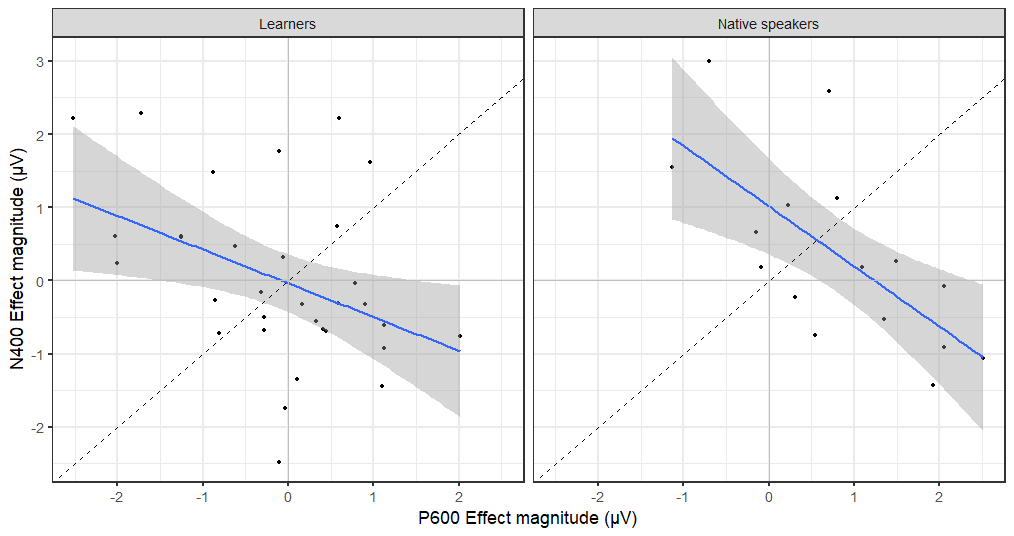
\includegraphics[width=5.1063in,height=2.6984in,width=\textwidth]{pelissier-img001.png}

\end{center}
\end{listWWNumxxlevelii}
\end{listWWNumxxleveli}
\begin{styleStandard}
\textbf{Figure 1: Correlation between N400 and P600 effect magnitudes for learners and native speakers}
\end{styleStandard}

\begin{styleStandard}
The first step was to examine the correlation between the N400 effect and the P600 effect in learners and native speakers, in order to assess whether participants exhibited one or the other effect instead of the expected biphasic pattern. There was indeed a significant negative correlation between the presence of a P600 and an N400 effect among learners (\textit{r }= -0.41, \textit{t}(30) = -2.49, \textit{p }{\textless} .05) and native speakers (\textit{r }= -0.68, \textit{t}(14) = -3.50, \textit{p }{\textless} .01), which is illustrated in Figure 1, where the blue line shows the best linear approximation for the correlation with a 95\% confidence interval. This shows that, consistent with previous studies, most participants exhibited either an N400 (participants to the left/above the dashed line, which represents equivalent N400 and P600 effects) or a P600 (participants to the right/below the dashed line) but not both. This can also be seen in Figure 2, which shows ERP waveforms for P600-dominant and N400-dominant native speakers and learners at Pz, a midline parietal electrode. Note that for P600-dominant learners, there appears to be a separate early positivity in the time window of the N400 before the P600, which suggests the engagement of attention-related mechanisms. The pattern for the native speakers is unusual in that the waveform in the correct condition contains a long-lasting negativity starting from around 400ms, which could reflect the cost of maintaining the critical word in memory to judge whether the sentence was acceptable. It is also worth noting that the N400 effect in the N400-dominant group seems to start right before the critical morpheme. This is hard to explain as this means that the difference started before the critical violation. A possible explanation is that there were some slight acoustic differences in the pronunciation of the verbs with and without the morpheme which these participants picked up on and which helped them anticipate the correctness of the word. 
\end{styleStandard}

\begin{center}
 [Warning: Image ignored] % Unhandled or unsupported graphics:
%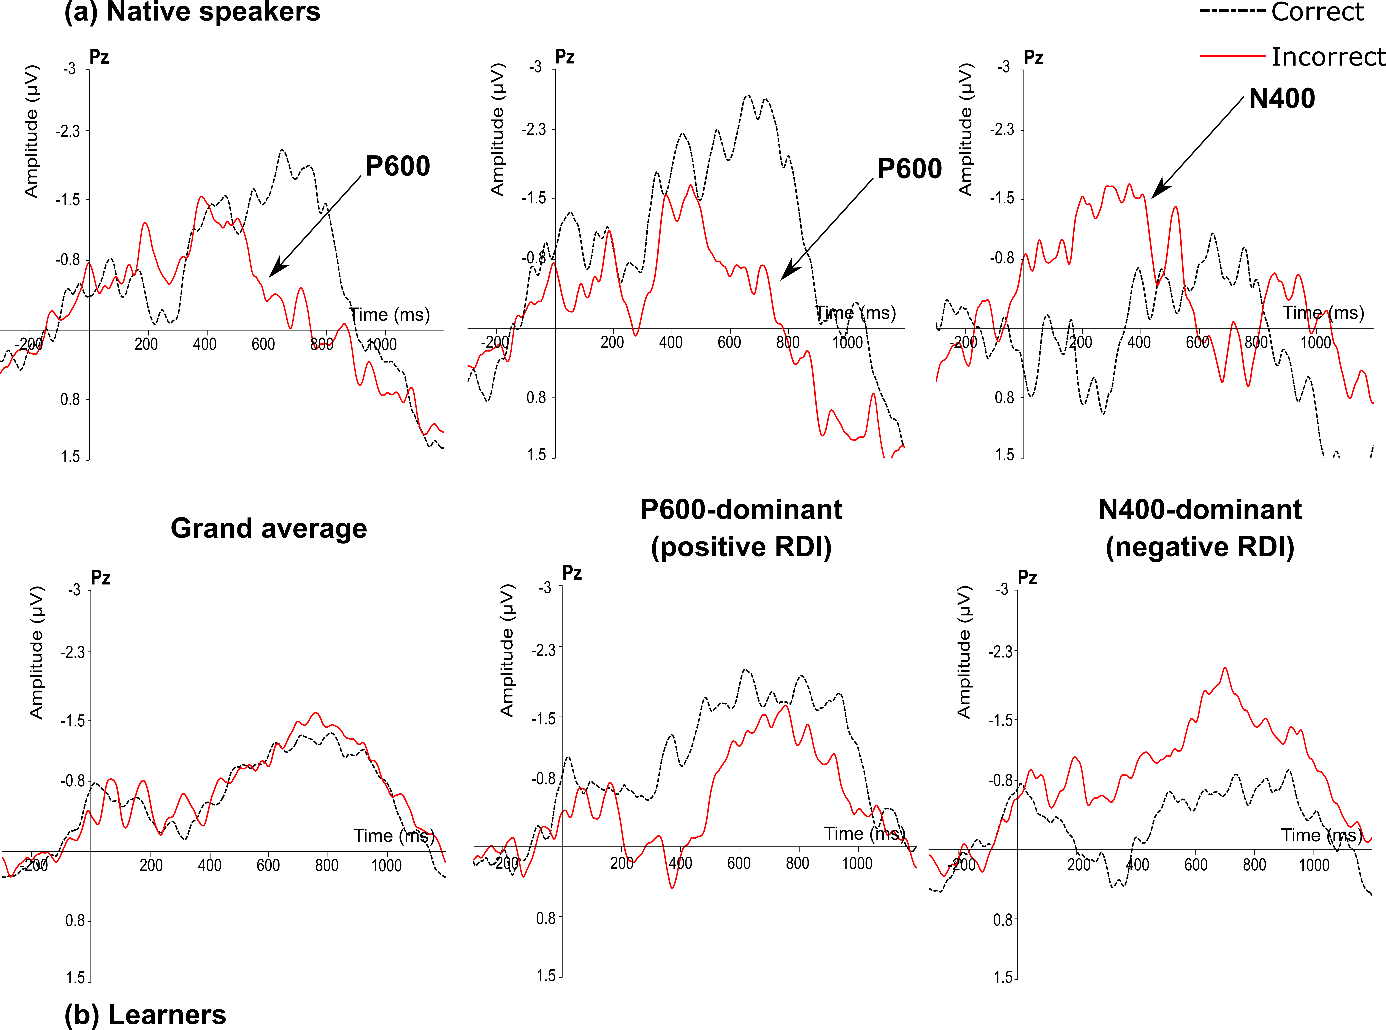
\includegraphics[width=6.3in,height=4.6819in,width=\textwidth]{pelissier-img002.png}

\end{center}
\begin{stylecaption}
\textbf{\textup{Figure 2:}}\textbf{ }\textbf{\textup{ERP waveforms to Correct (black dashed line) and Incorrect (red solid line) stimuli per group (Native speakers vs. Learners) for all participants and both RDI subgroups (P600-dominant and N400-dominant) at electrode Pz (midline parietal electrode)}}
\end{stylecaption}

\begin{styleStandard}
The second step was to evaluate the effect of the most studied predictor on GJT response magnitude – proficiency. A sensitivity index (\textit{d[2032?]} score) was computed for performance on the critical sentences – it is therefore a measure of structure-specific proficiency. There was a significant \textit{d[2032?] }difference between the two groups (\textit{t}(46) = -8.25, \textit{p }{\textless} 0.001): Learners were less proficient (\textit{M }= 0.80, \textit{SD }= 1.11) than native speakers (\textit{M }= 3.30, \textit{SD }= 0.70). There was no significant correlation between the amplitude of the P600 effect and proficiency for all participants combined (\textit{r} = 0.18, \textit{t}(46) = 1.21, \textit{p }{\textgreater} .2), nor when learners and native speakers were examined separately (Learners: \textit{r} = -0.19, \textit{t}(30) = -1.04, \textit{p }{\textgreater} .3; Natives: \textit{r} = -0.34, \textit{t}(14) = -1.33, \textit{p} {\textgreater} .2). However, there was a general positive correlation between the amplitude of the N400 effect and the \textit{d[2032?]} score (\textit{r }= 0.38, \textit{t}(46) = 2.80, \textit{p }{\textless} \ 0.01, see Figure 3). Participants who were more adept at detecting critical violations were thus more likely to exhibit an N400 than a P600. This s goes in the opposite direction from what we normally expect, which is that more proficient participants (especially as evaluated on a task that targets explicit knowledge like the GJT does) will show a P600 following syntactic violations. A separate correlation test for grammatical items revealed a similar positive correlation (\textit{r }= 0.36, \textit{t}(46) = 2.58, \textit{p }{\textless} \ 0.05): 
\end{styleStandard}

\begin{center}
 [Warning: Image ignored] % Unhandled or unsupported graphics:
%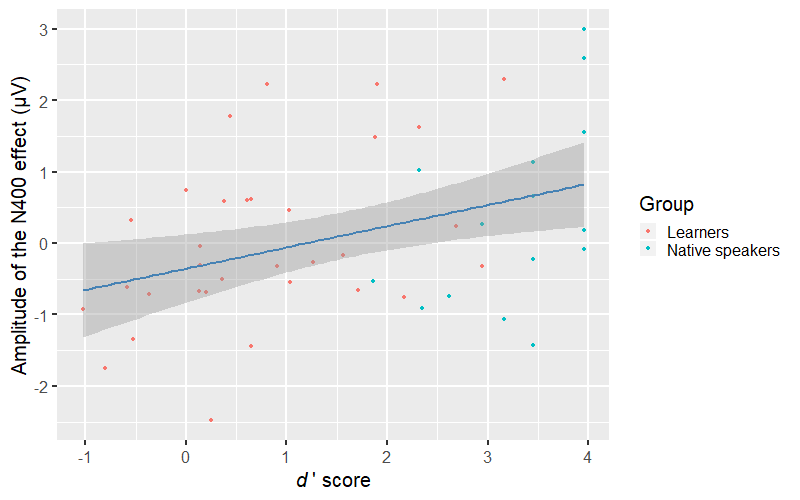
\includegraphics[width=4.198in,height=2.6236in,width=\textwidth]{pelissier-img003.png}

\end{center}
\begin{stylecaption}
\textbf{\textup{Figure 3: Amplitude of the N400 effect as a function of the }}\textbf{d[2032?]}\textbf{\textup{ score}}
\end{stylecaption}

\begin{styleStandard}
Participants who accepted more correct items exhibited a larger N400, while the correlation with ungrammatical items neared significance (\textit{r }= 0.27, \textit{t}(46) = 1.91, \textit{p }= 0.06), which is even more unexpected. \ When groups were examined separately, the correlation between the \textit{d[2032?]} score and the amplitude of the N400 effect was significant for learners (\textit{r }= 0.46, \textit{t}(30) = 2.82, \textit{p }{\textless} 0.01) but not for native speakers. It is interesting to note that there was no significant difference in the amplitude of the N400 between the two groups (\textit{t}(46) {\textless} 1) but a difference in the amplitude of the P600 effect (\textit{t}(46) = -2.89, \textit{p }{\textless} .01): Native speakers had a much larger P600 effect (\textit{M }= 0.81, \textit{SD }= 1.05) than learners, who did not exhibit a reliable P600 in response to violations (\textit{M }= -0.12, \textit{SD }= 1.06). \ Native speakers were more proficient and showed a significant P600 as a group, but among learners, more proficient participants tended to exhibit a larger N400. 
\end{styleStandard}

\begin{styleStandard}
The RMI was also computed. However, the correlation between RMI and \textit{d[2032?]} score did not reach significance (\textit{r }= 0.24, \textit{t}(46) = 1.71, \textit{p }= .09). There was no significant difference in RMI between the two groups (t(46) {\textless} 1; \textit{M}\textsubscript{Natives} = 1.61 µV, \textit{SD}\textsubscript{Natives} = 0.87 µV ; \textit{M}\textsubscript{Learners }= 1.37 µV, \textit{SD}\textsubscript{Learners }= 0.76 µV), despite the difference in proficiency (as reflected by the \textit{d[2032?]} score). In our case, the results were thus best explained by a simple relationship between the amplitude of the N400 and proficiency, rather than by a link between proficiency and the magnitude of the response in general. 
\end{styleStandard}

\begin{styleStandard}
These findings are surprising, as proficiency has previously been associated with a larger P600 amplitude or a more positive RMI in general. Native speakers’ performance was at ceiling, with a mean accuracy of 92.81\% (\textit{SD }= 14.60\%) on grammatical items and 95.31\% (\textit{SD }= 10.24\%) on ungrammatical items – with a median at 100\% for both. However, there was much more variability among learners: They did relatively well on grammatical items (\textit{M }= 79.06\%, \textit{SD }= 15.37\%, \textit{median }= 85\%, \textit{range }= 50-100\%) but were much less accurate on ungrammatical sentences (\textit{M }= 45\%, \textit{SD} = 27.85\%), \textit{median }= 35\%, \textit{range }= 5-100\%). For them, better proficiency was associated with a more negative-going response. This may be due to their overall proficiency in English, which was lower-intermediate. At this proficiency level, it is not uncommon for learners to exhibit an N400 after syntactic violations. They may have only reached the second stage of Steinhauer et al.’s (2009) model: After showing no response at all to syntactic violations, relatively more proficient learners show an N400 effect, which will evolve into a P600 with proficiency, like the one native speakers exhibit as a group.
\end{styleStandard}

\begin{listWWNumxxleveli}
\item 
\begin{listWWNumxxlevelii}
\item 
\begin{styleListParagraph}
\textbf{Individual differences: Response dominance}
\end{styleListParagraph}
\end{listWWNumxxlevelii}
\end{listWWNumxxleveli}
\begin{styleStandard}
The next step was to look at the Response Dominance Index. There was no significant difference in RDI between the two groups (\textit{t}(46) {\textless} 1). The RDI was also not correlated with the \textit{d[2032?]} score when participants were grouped together (\textit{t}(46) {\textless} 1). However, for learners, the RDI correlated with the \textit{d[2032?]} score (\textit{r }= -0.39, \textit{t}(30) = -2.33, \textit{p }{\textless} .05), which is consistent with the relationship that was found between the N400 effect and proficiency: More accurate participants were more likely to exhibit a negative-going effect rather than a P600. This correlation was driven by the performance on grammatical items, which was itself correlated with the RDI (\textit{r }= -0.36, \textit{t}(30) = -2.14, \textit{p }= .04). The processing of grammatical items is thought to engage implicit knowledge (Roehr-Brackin 2015), and it is worth noting that participants trained implicitly on artificial languages in studies by Morgan-Short et al. (2010; 2012) also exhibit an N400 at an intermediate proficiency level. 
\end{styleStandard}

\begin{styleStandard}
For native speakers however, the RDI-\textit{d[2032?]} correlation did not reach significance (\textit{r }= -0.44, \textit{t}(14) = -1.84, \textit{p }= .09). To understand this unexpected finding, one must keep in mind that during the EEG recording, participants did not complete the GJT but a semantic acceptability judgment task. I noticed that native speakers had difficulties with that task, specifically with ignoring grammatical incongruities in semantically acceptable sentences. Although their performance on the GJT was at ceiling, it is possible that their performance on the EEG task influenced the type of processing strategies they engaged in. To test this hypothesis, I computed a semantic \textit{dv} from the semantic acceptability task\footnote{\textrm{ In the semantic }\textrm{\textit{d[2032?]}}\textrm{, hits were sentences correctly identified as semantically correct, which could contain a syntactic violation. Sentences containing a semantic violation were fillers, and always syntactically correct.}}, reflecting how well native speakers managed to focus on the semantic aspect of sentences. The semantic \textit{d[2032?]} does not provide a measure of structure-specific proficiency, which is why the \textit{d[2032?]} of the GJT was used in the original analyses. \ Participants with a high semantic \textit{d[2032?] }score accepted sentences containing a grammatical violation but no semantic incongruity, while participants with a low semantic \textit{d[2032?]} score tended to reject ungrammatical items as semantically unacceptable. There was a strong correlation between the RDI and the semantic \textit{d[2032?]} score (\textit{r }= -0.56, \textit{t}(30) = -3.74, \textit{p }{\textless} .001): Participants who had a lower semantic \textit{d[2032?]} and thus focused more on the grammatical aspects of the stimuli had a more positive RDI and therefore exhibited a P600. Following this, I divided all participants (native speakers and learners) into two groups corresponding to a high or low semantic \textit{d[2032?]}.\footnote{ \textrm{The chosen splitting point was the median, as Hartigan’s dip test for unimodality did not reveal a multimodal distribution of the data (}\textrm{\textit{D}}\textrm{=0.03, }\textrm{\textit{p}}\textrm{{\textgreater}.1).}} A \textit{t}{}-test comparison between the two groups revealed that participants who had a lower semantic \textit{d[2032?]} also showed a larger (and positive) RDI (\textit{t}(157) = 3.64, \textit{p }{\textless} .001; \textit{M}\textsubscript{LowSemD}\textit{\textsubscript{[2032?]}}\textsubscript{ }\ = 0.37 µV, \textit{SD}\textsubscript{LowSemD}\textit{\textsubscript{[2032?]}}\textsubscript{ }= 1.21 µV;\textit{ M}\textsubscript{HighSemD}\textit{\textsubscript{[2032?]}}\textsubscript{ }= -0.38 µV, \textit{SD}\textsubscript{HighSemD}\textit{\textsubscript{[2032?]}}\textsubscript{ }= 1.39 µV). Rather than group membership (learners vs. native speakers), what seems to have influenced the type of electrophysiological response the most is participants’ attitude on the task and the strategy they chose to adopt. This is in line with the hypothesis that even native speakers do not all use the same mechanisms to process language. Participants who had difficulties ignoring the grammatical incongruities present in the input exhibited a P600 in response to the violations, because their attention was attracted to them and because they used combinatorial mechanisms even when processing language for meaning. On the contrary, participants who had a high semantic \textit{d[2032?]} successfully ignored grammatical violations to only reject semantically unacceptable sentences. In the case of learners, this success might simply be a correlate of the fact that they had great difficulties detecting violations, as their performance on the GJT suggests. However, there was no correlation between the semantic \textit{d[2032?]} and the capacity to detect violations (as measured by the performance on ungrammatical items; \textit{t}(126) {\textless} 1), so learners who obtained a high semantic \textit{d[2032?]} did not reach it just because they could not perceive the ungrammaticalities. There is no doubt that native speakers perceived the violations; those who performed well on the semantic acceptability task did so because they focused more on the lexico-semantic aspects of language, which is consistent with the fact that they exhibited much larger N400 effects.
\end{styleStandard}

\begin{styleStandard}
The task completed by participants during EEG data acquisition may well influence the RDI. Commonly used GJTs focus attention on form and may increase the likelihood of observing a P600, especially when stimuli are presented with the traditional and yet very artificial method of the rapid serial visual presentation. Tanner (2019) found similar results to those previously reported with his more ecological self-paced reading presentation – but with a simultaneous GJT. In my experiment, I had participants process stimuli for meaning instead of form, which let them use slightly more natural processing strategies. Not all language users grant the same importance to grammar in their native language, and this is evident from the results of our individual differences analyses. When given a choice, some people have no difficulties ignoring ungrammatical sentences, because they use other cues – lexico-semantic cues, as it appears – to interpret meaning, while others cannot do without combinatorial syntactic processes. Unfortunately, I do not have data concerning the number of left-handed close relatives of our native speakers, but this parameter may explain the differences in processing strategies (Grey et al. 2017). Using a less explicit task than a GJT proved to be of interest for studying individual differences, as it brought forth differences in strategies used to process meaning and not just form. 
\end{styleStandard}

\begin{listWWNumxxleveli}
\item 
\begin{styleListParagraph}
\textbf{Conclusion}
\end{styleListParagraph}
\end{listWWNumxxleveli}
\begin{styleStandard}
Comparing the electrophysiological correlates of language processing between learners and native speakers is proving difficult due to a high degree of individual variability even among native speakers. The traditional biphasic pattern of the LAN (or N400) followed by a P600 seems not to be representative of most individuals’ responses to morphosyntactic violations – our data extend findings obtained with agreement and phrase structure violations to tense morphology incongruities. The RMI did not prove a valuable measure for our data: Proficiency was associated with a larger amplitude of the N400 effect specifically. More research is needed to determine why in some cases proficiency is associated with the amplitude of a specific component (e.g. Tanner et al. 2009; 2013; White et al. 2012), whereas at other times it is reflected by the general amplitude of the response. The RDI is a useful way of qualifying the type of response elicited by the violations, which reflects the strategy recruited by language users. Response dominance has long been indirectly associated with learners’ proficiency, with models proposing an evolution from no response to an N400 and finally a P600 (Steinhauer et al. 2009). In our data, the RDI was directly associated with proficiency – among our group of intermediate learners, which can be hypothesized to be at the intermediate stage, more accurate learners exhibited more negative responses. But the most significant predictor in our case was participants’ strategy to complete the task, as measured by the performance on the semantic acceptability judgment task. 
\end{styleStandard}

\begin{styleStandard}
Individual differences among native speakers question the traditional syntax-first model (e.g. Friederici 2002) – there is not one single processing route that is nativelike, even when processing language for meaning and not to monitor grammatical incongruities. An important next step will therefore be to understand why this is the case and where the variability comes from: Is it random, or linked to genetic or environmental factors? Using artificial languages might be profitable to that end: Is individual variability as prevalent when all participants have learned the language in the exact same context and used it for the exact same purpose? \ A related open issue is how stable this individual variability is, over time (over several repeated sessions) but also across structures. Tanner \& van Hell (2014) found a correlation between the RDIs following two types of violations (subject-verb agreement and verb tense, i.e., missing or superfluous –\textit{ing} ending on the main verb), but more studies directly comparing RDIs across different but comparable structures are needed. Variable learner data cannot be fully interpreted without a good understanding of what drives the variability among native speakers.
\end{styleStandard}

\begin{styleStandard}
Another important issue will be to isolate the actual impact of the task on individual variability. Do we observe different processing strategies because of different task-solving strategies, or do native speakers resort to different processing mechanisms in everyday language use? Experiments comparing ERPs to the same structure while completing different tasks, such as acceptability judgments but also priming studies or comprehension questions, should be run to investigate this question. The development of existing technologies also offers new research perspectives – there are now smaller and cheaper EEGs that can be used outside of the lab, to study language in interaction for example. Even though it will be a challenge to obtain data that are controlled enough to do ERP analyses, these \ new devices will make it possible to study language processing in more ecological settings, which in turn may shed some light on the origins of individual variability in a less task-dependent way. In the meantime, when interpreting learner data, one must keep in mind the possible influence of the specific task on the observed results. 
\end{styleStandard}

\begin{styleStandard}
The absence of a clear native-speaker norm means that we cannot clearly interpret data as nativelike or not. Identifying the sources of individual variability among native speakers may allow us to compare more similar populations across native speakers and non-native speakers (e.g., right-handed speakers with no left-handed blood relatives), but that is quite restrictive and we need to go beyond what is eminently nativelike to question what makes processing strategies different at high proficiency. If we cannot clearly determine whether proficient language learners use the same mechanisms as native speakers, we might still be able to investigate whether they use the same range of mechanisms, and whether the same factors affect which processes are recruited and when. 
\end{styleStandard}

\begin{styleStandard}
\textbf{Acknowledgments }
\end{styleStandard}

\begin{styleStandard}
The experiment was funded by an Institut Universitaire de France grant awarded to Dr Emmanuel Ferragne.
\end{styleStandard}

\begin{styleStandard}
\textbf{References}
\end{styleStandard}

\begin{styleStandard}
Alemán Bañón, José \& Fiorentino, Robert \& Gabriele, Alison. 2014. Morphosyntactic processing in advanced second language (L2) learners: An event-related potential investigation of the effects of L1–L2 similarity and structural distance. \textit{Second Language Research} 30(3). 275–306.
\end{styleStandard}

\begin{styleStandard}
Alemán Bañón, José \& Miller, David \& Rothman, Jason. 2017. Morphological variability in second language learners: An examination of electrophysiological and production data. \textit{Journal of Experimental Psychology: Learning, Memory, and Cognition} 43(10). 1509–1536.
\end{styleStandard}

\begin{styleStandard}
Astésano, Corine \& Besson, Mireille \& Alter, Kai. 2004. Brain potentials during semantic and prosodic processing in French. \textit{Cognitive Brain Research} 18(2). 172–184.
\end{styleStandard}

\begin{styleStandard}
Barber, Horacio \& Carreiras, Manuel. 2005. Grammatical gender and number agreement in Spanish: An ERP comparison. \textit{Journal of Cognitive Neuroscience} 17(1). 137–153.
\end{styleStandard}

\begin{styleStandard}
Bates, Douglas \& Mächler, Martin \& Bolker, Ben \& Walker, Steve. Fitting linear mixed-effects models using lme4. \textit{Journal of Statistical Software} 67(1). 1–48.
\end{styleStandard}

\begin{styleStandard}
Batterink, Laura \& Neville, Helen. 2013. Implicit and explicit second language training recruit common neural mechanisms for syntactic processing. \textit{Journal of Cognitive Neuroscience} 25(6). 936–951.
\end{styleStandard}

\begin{styleStandard}
Birdsong, David. 2006. Age and second language acquisition and processing: A selective overview. \textit{Language Learning} 56(1). 9–49.
\end{styleStandard}

\begin{styleStandard}
Bond, Kristi \& Gabriele, Alison \& Fiorentino, Robert \& Alemán Bañón, José. 2011. Individual differences and the role of the L1 in L2 processing: An ERP investigation. In Tanner, Darren \& Herschensohn, Julia (eds), \textit{Proceedings of the 11th Generative Approaches to Second Language Acquisition Conference (GASLA 2011) }17–29. Somerville, MA: Cascadilla Proceedings Project.
\end{styleStandard}

\begin{styleStandard}
Bowden, Harriet Wood \& Steinhauer, Karsten \& Sanz, Cristina \& Ullman, Michael T. 2013. Native-like brain processing of syntax can be attained by university foreign language learners. \textit{Neuropsychologia} 51(13). 2492–2511.
\end{styleStandard}

\begin{styleStandard}
Caffarra, Sendy \& Molinaro, Nicola \& Davidson, Doug \& Carreiras, Manuel. 2015. Second language syntactic processing revealed through event-related potentials: An empirical review. \textit{Neuroscience and Biobehavioral Reviews} 51. 31–47.
\end{styleStandard}

\begin{styleStandard}
Chen, Lang \& Shu, Hua \& Liu, Youyi \& Zhao, Jingjing \& Li, Ping. 2007. ERP signatures of subject–verb agreement in L2 learning. \textit{Bilingualism: Language and Cognition} 10(2). 161–174.
\end{styleStandard}

\begin{styleStandard}
Clahsen, Harald \& Felser, Claudia. 2006. Grammatical processing in language learners. \textit{Applied Psycholinguistics}. 27(01). 3–42.
\end{styleStandard}

\begin{styleStandard}
Clahsen, Harald \& Felser, Claudia. 2018.~Some notes on the Shallow Structure Hypothesis.~S\textit{tudies in Second Language Acquisition.}~40(3). 693-706. 
\end{styleStandard}

\begin{styleStandard}
DeLong, Katherine A. \& Quante, Laura \& Kutas, Marta. 2014. Predictability, plausibility, and two late ERP positivities during written sentence comprehension. \textit{Neuropsychologia} 61. 150–162.
\end{styleStandard}

\begin{styleStandard}
DeLong, Katherine A. \& Urbach, Thomas P. \& Kutas, Marta. 2005. Probabilistic word pre-activation during language comprehension inferred from electrical brain activity. \textit{Nature Neuroscience} 8(8). 1117–1121.
\end{styleStandard}

\begin{styleStandard}
Fabiani, Monica \& Gratton, Gabriele \& Federmeier, Kara D. 2007. Event-related brain potentials: Methods, theory, and applications. In Cacioppo, John, Tassinary, Louis G. \& Berntson, Gary G. (eds), \textit{Handbook of psychophysiology}, 85–119. Cambridge: Cambridge University Press.
\end{styleStandard}

\begin{styleStandard}
Faretta-Stutenberg, Mandy \& Morgan-Short, Kara. 2018. The interplay of individual differences and context of learning in behavioral and neurocognitive second language development. \textit{Second Language Research }34(1). 67–101.
\end{styleStandard}

\begin{styleStandard}
Federmeier, Kara D. 2007. Thinking ahead: The role and roots of prediction in language comprehension. \textit{Psychophysiology} 44(4). 491–505.
\end{styleStandard}

\begin{styleStandard}
Federmeier, Kara D. \& Kutas, Marta. 1999. A rose by any other name: Long-term memory structure and sentence processing. \textit{Journal of Memory and Language} 41(4). 469–495.
\end{styleStandard}

\begin{styleStandard}
Foucart, Alice \& Frenck-Mestre, Cheryl. 2010. Grammatical gender processing in L2: Electrophysiological evidence of the effect of L1–L2 syntactic similarity. \textit{Bilingualism: Language and Cognition} 14(3). 379–399.
\end{styleStandard}

\begin{styleStandard}
Foucart, Alice \& Frenck-Mestre, Cheryl. 2012. Can late L2 learners acquire new grammatical features? Evidence from ERPs and eye-tracking. \textit{Journal of Memory and Language} 66(1). 226–248.
\end{styleStandard}

\begin{styleStandard}
Foucart, Alice \& Martin, Clara D. \& Moreno, Eva M. \& Costa, Albert. 2014. Can bilinguals see it coming? Word anticipation in L2 sentence reading. \textit{Journal of Experimental Psychology: Learning, Memory, and Cognition} 40(5). 1461–1469.
\end{styleStandard}

\begin{styleStandard}
Friederici, Angela D. 2002. Towards a neural basis of auditory sentence processing. \textit{Trends in Cognitive Sciences}. 6(2). 78–84.
\end{styleStandard}

\begin{styleStandard}
Friederici, Angela D. \& Pfeifer, Erdmut \& Hahne, Anja. 1993. Event-related brain potentials during natural speech processing: Effects of semantic, morphological and syntactic violations. \textit{Cognitive Brain Research} 1(3). 183–192.
\end{styleStandard}

\begin{styleStandard}
Fromont, Lauren A. \& Royle, Phaedra \& Steinhauer, Karsten. 2012. On-line processing of French syntactic word categories in native speakers and late L2 learners: An ERP study. In Name of volume editor \textit{CUNY}, 5–6. Cambridge, MA: Name of publisher.
\end{styleStandard}

\begin{styleStandard}
Gillon-Dowens, Margaret \& Guo, Taomei \& Guo, Jingjing \& Barber, Horacio \& Carreiras, Manuel. 2011. Gender and number processing in Chinese learners of Spanish – Evidence from event-related potentials. \textit{Neuropsychologia} 49(7). 1651–1659.
\end{styleStandard}

\begin{styleStandard}
Gillon-Dowens, Margaret \& Vergara, Marta \& Barber, Horacio \& Carreiras, Manuel. 2010. Morphosyntactic processing in late second-language learners. \textit{Journal of Cognitive Neuroscience} 22(8). 1870–1887.
\end{styleStandard}

\begin{styleStandard}
Grey, Sarah \& Tanner, Darren \& van Hell, Janet G. 2017. How right is left? Handedness modulates neural responses during morphosyntactic processing. \textit{Brain Research} 1669. 27–43.
\end{styleStandard}

\begin{styleStandard}
Gunter, Thomas C. \& Friederici, Angela D. \& Schriefers, Herbert. 2000. Syntactic gender and semantic expectancy: ERPs reveal early autonomy and late interaction. \textit{Journal of Cognitive Neuroscience} 12(4). 556–568.
\end{styleStandard}

\begin{styleStandard}
Guo, Jingjing \& Guo, Taomei \& Yan, Yan \& Jiang, Nan \& Peng, Danling. 2009. ERP evidence for different strategies employed by native speakers and L2 learners in sentence processing. \textit{Journal of Neurolinguistics} 22(2). 123–134.
\end{styleStandard}

\begin{styleStandard}
Hahne, Anja \& Mueller, Jutta L. \& Clahsen, Harald. 2006. Morphological processing in a second language: Behavioral and event-related brain potential evidence for storage and decomposition. \textit{Journal of Cognitive Neuroscience} 18(1). 121–134.
\end{styleStandard}

\begin{styleStandard}
Hakuta, Kenji \& Bialystok, Ellen \& Wiley, Edward. 2003. Critical evidence. \textit{Psychological Science} 14(1). 31–38.
\end{styleStandard}

\begin{styleStandard}
Isel, Frédéric. 2017. Apport de l’électro-encéphalographie à l’étude des atypies du traitement du langage: Apport de la psycholinguistique et des neurosciences cognitives. In Bogliotti, Caroline \& Isel, Frédéric \& Lacheret-Dujour, Anne (eds), \textit{Atypies langagières de l’enfance à l’âge adulte}, 149–192. Paris: De Boeck Supérieur.
\end{styleStandard}

\begin{styleStandard}
Isel, Frédéric \& Hahne, Anja \& Maess, Burkhard \& Friederici, Angela D. 2007. Neurodynamics of sentence interpretation: ERP evidence from French. \textit{Biological Psychology} 74(3). 337–346.
\end{styleStandard}

\begin{styleStandard}
Isel, Frédéric \& Kail, Michèle. 2018. Morphosyntactic integration in French sentence processing: Event-related brain potentials evidence. \textit{Journal of Neurolinguistics} 46. 23–36.
\end{styleStandard}

\begin{styleStandard}
Kaan, Edith. 2007. Event-related potentials and language processing: A brief overview. \textit{Language and Linguistics Compass} 1(6). 571–591.
\end{styleStandard}

\begin{styleStandard}
Kim, Albert E. \& Oines, Leif \& Miyake, Akira. 2018. Individual differences in verbal working memory underlie a tradeoff between semantic and structural processing difficulty during language comprehension: An ERP investigation. \textit{Journal of Experimental Psychology: Learning, Memory, and Cognition} 44(3). 406–420.
\end{styleStandard}

\begin{styleStandard}
Kotz, Sonja A. 2009. A critical review of ERP and fMRI evidence on L2 syntactic processing. \textit{Brain and Language} 109(2–3). 68–74.
\end{styleStandard}

\begin{styleStandard}
Kotz, Sonja A. \& Holcomb, Phillip J. \& Osterhout, Lee. 2008. ERPs reveal comparable syntactic sentence processing in native and non-native readers of English. \textit{Acta Psychologica} 128(3). 514–527.
\end{styleStandard}

\begin{styleStandard}
Kutas, Marta \& Hillyard, Steven A. 1980. Event-related brain potentials to semantically inappropriate and surprisingly large words. \textit{Biological Psychology} 11(2). 99–116.
\end{styleStandard}

\begin{styleStandard}
Kutas, Marta \& DeLong, Katherine A. \& Smith, Nathaniel J. 2011. A look around at what lies ahead: Prediction and predictability in language processing. In Bar, M\textit{full first name here please}. (ed.), \textit{Predictions in the brain: Using our past to generate a future}, 190–207. Oxford: Oxford University Press.
\end{styleStandard}

\begin{styleStandard}
Lenth, Russel. 2019.\textit{ emmeans: Estimated marginal means, aka least-square means. }R package version 1.4.1. (https://CRAN.R-project.org/package=emmeans) [I couldn'd find this reference in the main text.]
\end{styleStandard}

\begin{styleStandard}
Luck, Steven J. 2014. \textit{An introduction to the event-related potential technique}, 2\textsuperscript{nd} edition. Cambridge, MA: MIT Press.
\end{styleStandard}

\begin{styleStandard}
Martín-Loeches, Manuel \& Muñoz, Francisco \& Casado, Pilar \& Melcón, A. [Add full name] \& Fernández-Frías, C. [Full author name] 2005. Are the anterior negativities to grammatical violations indexing working memory? \textit{Psychophysiology} 42(5). 508–519.
\end{styleStandard}

\begin{styleStandard}
McLaughlin, Judith \& Osterhout, Lee \& Kim, Albert. 2004. Neural correlates of second-language word learning: Minimal instruction produces rapid change. \textit{Nature Neuroscience} 7. 703–704.
\end{styleStandard}

\begin{styleStandard}
McLaughlin, Judith \& Tanner, Darren \& Pitkänen, Ilona \& Frenck-Mestre, Cheryl \& Inoue, Kayo \& Valentine, Geoffrey \& Osterhout, Lee.2010. Brain potentials reveal discrete stages of L2 grammatical learning. \textit{Language Learning} 60. 123–150.
\end{styleStandard}

\begin{styleStandard}
Mehravari, Alison S. \& Emmorey, Karen \& Prat, Chantel S. \& Klarman, Lindsay \& Osterhout, Lee. 2017. Brain-based individual difference measures of reading skill in deaf and hearing adults. \textit{Neuropsychologia} 101. 153–168.
\end{styleStandard}

\begin{styleStandard}
Meulman, Nienke \& Wieling, Martijn \& Sprenger, Simone A. \& Stowe, Laurie A. \& Schmid, Monika S. 2015. Age effects in L2 grammar processing as revealed by ERPs and how (not) to study them. \textit{PloS One} 10(12). e0143328.
\end{styleStandard}

\begin{styleStandard}
Molinaro, Nicola \& Barber, Horacio A. [NB: sometimes cited as Horacio and sometimes as Horacio A.] \& Carreiras, Manuel. 2011. Grammatical agreement processing in reading: ERP findings and future directions. \textit{Cortex} 47(8). 908–930.
\end{styleStandard}

\begin{styleStandard}
Molinaro, Nicola \& Vespignani, Francesco \& Job, Remo. 2008. A deeper reanalysis of a superficial feature: An ERP study on agreement violations. \textit{Brain Research} 1228. 161–176.
\end{styleStandard}

\begin{styleStandard}
Morgan-Short, Kara \& Faretta-Stutenberg, Mandy \& Bartlett-Hsu, Laura. 2015. Contributions of event-related potential research to issues in explicit and implicit second language acquisition. In Rebuschat, Patrick (ed.), \textit{Implicit and explicit learning of languages}, 349–384. Amsterdam: John Benjamins.
\end{styleStandard}

\begin{styleStandard}
Morgan-Short, Kara \& Sanz, Cristina \& Steinhauer, Karsten \& Ullman, Michael T. 2010. Second language acquisition of gender agreement in explicit and implicit training conditions: An event-related potential study. \textit{Language Learning} 60(1). 154–193.
\end{styleStandard}

\begin{styleStandard}
Morgan-Short, Kara \& Steinhauer, Karsten \& Sanz, Cristina \& Ullman, Michael T. 2012. Explicit and implicit second language training differentially affect the achievement of native-like brain activation patterns. \textit{Journal of Cognitive Neuroscience} 24(4). 933–947.
\end{styleStandard}

\begin{styleStandard}
Mueller, Jutta L. \& Hirotani, Masako \& Friederici, Angela D. 2007. ERP evidence for different strategies in the processing of case markers in native speakers and non-native learners. \textit{BMC Neuroscience} 8(1). 18.
\end{styleStandard}

\begin{styleStandard}
Nakano, Hiroko \& Saron, Clifford \& Swaab, Tamara Y. 2010. Speech and span: Working memory capacity impacts the use of animacy but not of world knowledge during spoken sentence comprehension. \textit{Journal of Cognitive Neuroscience} 22(12). 2886–2898.
\end{styleStandard}

\begin{styleStandard}
Newman, Aaron J. \& Ullman, Michael T. \& Pancheva, Roumyana \& Waligura, Diane L. \& Neville, Helen J. 2007. An ERP study of regular and irregular English past tense inflection. \textit{NeuroImage} 34(1). 435–445.
\end{styleStandard}

\begin{styleStandard}
Newman, Aaron J. \& Tremblay, Antoine \& Nichols, Emily S. \& Neville, Helen J. \& Ullman, Michael T. 2012. The influence of language proficiency on lexical semantic processing in native and late learners of English. \textit{Journal of cognitive neuroscience} 24(5). 1205–1223.
\end{styleStandard}

\begin{styleStandard}
Ojima, Shiro \& Nakata, Hiroki \& Kakigi, Ryusuke. 2005. An ERP study of second language learning after childhood: Effects of proficiency. \textit{Journal of Cognitive Neuroscience}. 17(8). 1212–1228.
\end{styleStandard}

\begin{styleStandard}
Osterhout, Lee. 1997. On the brain response to syntactic anomalies: Manipulations of word position and word class reveal individual differences. \textit{Brain and Language} 59(3). 494–522.
\end{styleStandard}

\begin{styleStandard}
Osterhout, Lee \& Holcomb, Phillip J. 1992. Event-related brain potentials elicited by syntactic anomaly. \textit{Journal of Memory and Language} 31(6). 785–806.
\end{styleStandard}

\begin{styleStandard}
Osterhout, Lee \& McLaughlin, Judith \& Kim, Albert \& Greenwald, Ralf \& Inoue, Kayo. 2004. Sentences in the brain: Event-related potentials as real-time reflections of sentence comprehension and language learning. In Carreiras, Manuel \& Clifton Jr., Charles (eds), \textit{The on-line study of sentence comprehension: Eyetracking, ERP, and beyond}, 271–308. New York: Psychology Press.
\end{styleStandard}

\begin{styleStandard}
Osterhout, Lee \& Mclaughlin, Judy \& Pitkänen, Ilona \& Frenck-Mestre, Cheryl \& Molinaro, Nicola. 2006. Novice learners, longitudinal designs, and event-related potentials: A means for exploring the neurocognition of second language processing. \textit{Language Learning} 56. 199–230.
\end{styleStandard}

\begin{styleStandard}
Pakulak, Eric \& Neville, Helen J. 2010. Proficiency differences in syntactic processing of monolingual native speakers indexed by event-related potentials. \textit{Journal of Cognitive Neuroscience} 22(12). 2728–2744.
\end{styleStandard}

\begin{styleStandard}
Paradis, Michel. 2009. \textit{Declarative and procedural determinants of second languages}. Amsterdam: John Benjamins.
\end{styleStandard}

\begin{styleStandard}
Qi, Zhenghan \& Beach, Sara D. \& Finn, Amy S. \& Minas, Jennifer \& Goetz, Calvin \& Chan, Brian \& Gabrieli, John D.E. 2017. Native-language N400 and P600 predict dissociable language-learning abilities in adults. \textit{Neuropsychologia} 98. 177–191.
\end{styleStandard}

\begin{styleStandard}
R Core Team. 2019. \textit{R: A language and environment for statistical computing. }(Version 3.6.1.) Vienna: R foundation for statistical computing. [Cited as such also in the main text?]
\end{styleStandard}

\begin{styleStandard}
Roehr-Brackin, Karen. 2015. Explicit knowledge about language in L2 learning: A usage-based perspective. In Rebuschat, Patrick (ed.), \textit{Implicit and explicit learning of languages}, 117–138. Amsterdam: John Benjamins.
\end{styleStandard}

\begin{styleStandard}
Rossi, Sonja \& Gugler, Manfred F. \& Friederici, Angela D. \& Hahne, Anja. 2006. The impact of proficiency on syntactic second-language processing of German and Italian: Evidence from event-related potentials. \textit{Journal of Cognitive Neuroscience} 18(12). 2030–2048.
\end{styleStandard}

\begin{styleStandard}
Sassenhagen, Jona \& Schlesewsky, Matthias \& Bornkessel-Schlesewsky, Ina. 2014. The P600-as-P3 hypothesis revisited: Single-trial analyses reveal that the late EEG positivity following linguistically deviant material is reaction time aligned. \textit{Brain and Language} 137. 29–39.
\end{styleStandard}

\begin{styleStandard}
Schneider, Julie M. \& Abel, Alyson D. \& Ogiela, Diane A. \& Middleton, Anna E. \& Maguire, Mandy J. 2016. Developmental differences in beta and theta power during sentence processing. \textit{Developmental Cognitive Neuroscience} 19. 19–30.
\end{styleStandard}

\begin{styleStandard}
Steinhauer, Karsten. 2014. Event-related potentials (ERPs) in second language research: A brief introduction to the technique, a selected review, and an invitation to reconsider critical periods in L2. \textit{Applied Linguistics} 35(4). 393–417.
\end{styleStandard}

\begin{styleStandard}
Steinhauer, Karsten \& White, Erin J. \& Drury, John E. 2009. Temporal dynamics of late second language acquisition: Evidence from event-related brain potentials. \textit{Second Language Research} 25(1). 13–41.
\end{styleStandard}

\begin{styleStandard}
Tanner, Darren. 2019. Robust neurocognitive individual differences in grammatical agreement processing: A latent variable approach. \textit{Cortex} 111. 210–237.
\end{styleStandard}

\begin{styleStandard}
Tanner, Darren \& Inoue, Kayo \& Osterhout, Lee. 2012. \textit{Brain-based individual differences in on-line L2 sentence comprehension.} MS., Pennsylvania State University.
\end{styleStandard}

\begin{styleStandard}
Tanner, Darren \& Inoue, Kayo \& Osterhout, Lee. 2014. Brain-based individual differences in online L2 grammatical comprehension. \textit{Bilingualism: Language and Cognition} 17(02). 277–293.
\end{styleStandard}

\begin{styleStandard}
Tanner, Darren \& Mclaughlin, Judith \& Herschensohn, Julia \& Osterhout, Lee. 2013. Individual differences reveal stages of L2 grammatical acquisition: ERP evidence. \textit{Bilingualism: Language and Cognition} 16(Special Issue 2). 367–382.
\end{styleStandard}

\begin{styleStandard}
Tanner, Darren \& Osterhout, Lee \& Herschensohn, Julia. 2009. Snapshots of grammaticalization: Differential electrophysiological responses to grammatical anomalies with increasing L2 exposure. In Editor? \textit{BUCLD 33: Proceedings of the 33rd Boston University Conference on Language Development}, 528–539. Boston, MA: Cascadilla Press.
\end{styleStandard}

\begin{styleStandard}
Tanner, Darren \& van Hell, Janet G. 2014. ERPs reveal individual differences in morphosyntactic processing. \textit{Neuropsychologia} 56(1). 289–301.
\end{styleStandard}

\begin{styleStandard}
Tokowicz, Natasha \& MacWhinney, Brian. 2005. Implicit and explicit measures of sensitivity to violations in second language grammar: An event-related potential investigation. \textit{Studies in Second Language Acquisition} 27(2). 173–204.
\end{styleStandard}

\begin{styleStandard}
Tokowicz, Natasha \& Michael, Erica B. \& Kroll, Judith F. 2004. The roles of study-abroad experience and working-memory capacity in the types of errors made during translation. \textit{Bilingualism: Language and Cognition} 7(3). 255–272.
\end{styleStandard}

\begin{styleStandard}
van de Meerendonk, Nan \& Kolk, Herman H.J. \& Chwilla, Dorothee J. \& Vissers, Constance Th. W.M. 2009. Monitoring in language perception. \textit{Language and Linguistics Compass} 3(5). 1211–1224.
\end{styleStandard}

\begin{styleStandard}
van Hell, Janet G. \& Tokowicz, Natasha. 2010. Event-related brain potentials and second language learning: Syntactic processing in late L2 learners at different L2 proficiency levels. \textit{Second Language Research} 26(1). 43–74.
\end{styleStandard}

\begin{styleStandard}
Wampler, Emma K. 2017. \textit{Individual differences in grammatical error processing}. Seattle: University of Washington. (Doctoral dissertation.)
\end{styleStandard}

\begin{styleStandard}
Wampler, Emma K. \& Mclaughlin, Judith \& Osterhout, Lee. 2014. How gender, handedness, and L1 processing strategy influence L2 grammatical processing. \textit{In}: \textit{Society for the Neurobiology of Language}. Is this a collected volume? Proceedings? Please provide the name of the editor(s), the publisher, and the page numbers
\end{styleStandard}

\begin{styleStandard}
Weber-Fox, C. \& Neville, Helen. 1996. Maturational constraints on functional specializations for language processing: ERP and behavioral evidence in bilingual speakers. \textit{Journal of Cognitive Neuroscience} 8. 231–256.
\end{styleStandard}

\begin{styleStandard}
Weiss, Sabine \& Mueller, Horst M. \& Schack, Baerbel \& King, Jonathan W. \& Kutas, Martha \& Rappelsberger, Peter. 2005. Increased neuronal communication accompanying sentence comprehension. \textit{International Journal of Psychophysiology} 57(2). 129–141.
\end{styleStandard}

\begin{styleStandard}
White, Erin Jacquelyn \& Genesee, Fred \& Steinhauer, Karsten. 2012. Brain responses before and after intensive second language learning: Proficiency based changes and first language background effects in adult learners. \textit{PloS One} 7(12). e52318.
\end{styleStandard}

\begin{styleStandard}
Xue, Jin \& Yang, Jie \& Zhang, Jie \& Qi, Zhenhai \& Bai, Chen \& Qiu, Yinchen. 2013. An ERP study on Chinese natives’ second language syntactic grammaticalization. \textit{Neuroscience Letters} 534. 258–263.
\end{styleStandard}

\begin{styleStandard}
Zawiszewski, Adam \& Gutiérrez, Eva \& Fernández, Beatriz \& Laka, Itziar. 2011. Language distance and non-native syntactic processing: Evidence from event-related potentials. \textit{Bilingualism: Language and Cognition} 14(03). 400–411.
\end{styleStandard}

\end{document}
